\documentclass[a4paper]{article}

\def\nbook {All of Statistics: A Concise Course in Statistical Inference}
\def\nbookshort {All of Statistics}

% Shared preamble. The fallback lets the document build whether the working
% directory is its own folder or the project root.
\IfFileExists{headerallofstats.tex}{\input{headerallofstats}}{%%%%%%%%%%%%%%%%%%%%
% AUTHOR AND HEADER
% define \nbook
%%%%%%%%%%%%%%%%%%%%

\makeatletter
\ifx \nauthor\undefined
  \def\nauthor{David A. Lee}
\else
\fi

\author{\nbook \\ \small Solutions by \nauthor}
\date{}

%%%%%%%%%%%%%%%%%%%%
% PACKAGES
%%%%%%%%%%%%%%%%%%%%

\usepackage{alltt} 
\usepackage{amsfonts}
\usepackage{amsmath}
\usepackage{amssymb}
\usepackage{amsthm}
\usepackage{bm}
\usepackage{booktabs}
\usepackage{caption}
\usepackage{centernot}
\usepackage{enumitem}
\usepackage{fancyhdr}
\usepackage[T1]{fontenc}
\usepackage{graphicx}
% Images live in chap1/ ... chap8/ at the project root, while the documents that
% use them sit one level down (allofstats/, allofstatschap1/, ...). Listing both
% "./" and "../" lets a document keep writing \includegraphics{chap1/foo.eps}
% and still resolve it whether it is compiled from its own folder or from the
% project root.
\graphicspath{{./}{../}}
\usepackage{mathdots}
\usepackage{mathtools}
\usepackage{microtype}
\usepackage{multirow}
\usepackage{pdflscape}
\usepackage{pgfplots}
\pgfplotsset{compat=1.18}
\usepackage{siunitx}
\usepackage{slashed}
\usepackage{tabularx}
\usepackage{tikz}
\usepackage{titletoc}
\usepackage{tkz-euclide}
\usepackage[normalem]{ulem}
\usepackage{url}
\usepackage[all]{xy}
\usepackage{imakeidx}

% fonts
% use \textsf to change to Computer Modern Bright
\renewcommand{\sfdefault}{cmbr} % keeps default font Computer Modern Roman

% makeindex for table of contents
\makeindex[intoc, title=Index]
\indexsetup{othercode={\lhead{ Index }}}

% table of contents remove numbering
\setcounter{secnumdepth}{0}

% pagestyle
\pagestyle{fancyplain}

% header
\lhead{	\nouppercase{\leftmark} }
\ifx \nextra \undefined
  \rhead{
    \ifnum\thepage=1
    \else
      \nbookshort \  | \nauthor
    \fi}
\else
  \rhead{
    \ifnum\thepage=1
    \else
      \nbookshort (\nextra)
    \fi}
\fi

% proof environment

\newcommand{\prooffont}{\scshape}
\usepackage{xpatch}
\tracingpatches
\xpatchcmd{\proof}{\itshape}{\prooffont}{}{}

% Python environment (for typesetting Python code)

% Default fixed font does not support bold face
\DeclareFixedFont{\ttb}{T1}{txtt}{bx}{n}{8} % for bold
\DeclareFixedFont{\ttm}{T1}{txtt}{m}{n}{8}  % for normal

% Custom colors
\usepackage{color}
\definecolor{deepblue}{rgb}{0,0,0.5}
\definecolor{deepred}{rgb}{0.6,0,0}
\definecolor{deepgreen}{rgb}{0,0.5,0}

\usepackage{listings}

% Python style for highlighting
\newcommand\pythonstyle{\lstset{
language=Python,
basicstyle=\ttm,
morekeywords={self},              % Add keywords here
keywordstyle=\ttb\color{deepblue},
emph={MyClass,__init__},          % Custom highlighting
emphstyle=\ttb\color{deepred},    % Custom highlighting style
stringstyle=\color{deepgreen},
frame=tb,                         % Any extra options here
showstringspaces=false
}}


% Python environment
\lstnewenvironment{python}[1][]
{
\pythonstyle
\lstset{#1}
}
{}

% Python for external files
\newcommand\pythonexternal[2][]{{
\pythonstyle
\lstinputlisting[#1]{#2}}}

% Python for inline
\newcommand\pythoninline[1]{{\pythonstyle\lstinline!#1!}}

%%%%%%%%%%%%%
% FUNCTIONS %
%%%%%%%%%%%%%

\DeclarePairedDelimiter\abs{\lvert}{\rvert}%
\DeclarePairedDelimiter\norm{\lVert}{\rVert}%

%%%%%%%%%%%%%%%%%%%%
% DOCUMENT GEOMETRY
%%%%%%%%%%%%%%%%%%%%

\ifx \ntrim \undefined
\else
  \usepackage{geometry}
  \geometry{
	  papersize={379pt, 699pt},
	  textwidth=345pt,
	  left=17pt,
	  top=54pt,
	  right=17pt,
  }
\fi

% maketitle statement
\title{}
\ifx \nisofficial \undefined
\let\@real@maketitle\maketitle
\renewcommand{\maketitle}{\@real@maketitle\begin{center}\begin{minipage}[c]{0.9\textwidth}\centering\footnotesize All errors, typographical and substantive, and other offenses, are entirely my own.\end{minipage}\end{center}}
\else
\fi

%%%%%%%%%%%%%%%%%%%%
% THEOREMS
%%%%%%%%%%%%%%%%%%%%

%\theoremstyle{definition}
\newtheorem*{axiom}{Axiom}
\newtheorem*{claim}{Claim}
\newtheorem*{conjecture}{Conjecture}
\newtheorem*{cor}{Corollary}
%\newtheorem*{dfn}{Definition}
\newtheorem*{eg}{Example}
\newtheorem*{ex}{Exercise}
%\newtheorem*{lemma}{Lemma}
\newtheorem*{prop}{Proposition}
%\newtheorem*{thm}{Theorem}
\newtheorem*{remark}{Remark}
\newtheorem*{warning}{Warning}

%%%%%%%%%%%%%%%%%%%%
% FORMATTING AESTHETICS
%%%%%%%%%%%%%%%%%%%%

% itemize bullets
\renewcommand{\labelitemi}{-}
\renewcommand{\labelitemii}{$\circ$}
\renewcommand{\labelenumi}{(\roman{*})}

% new page section
\let\stdsection\section
\renewcommand\section{\newpage\stdsection}

%%%%%%%%%%%%%%%%%%%%
% \mathbb commands
%%%%%%%%%%%%%%%%%%%%

\newcommand{\C}{\mathbb{C}}
\newcommand{\N}{\mathbb{N}}
\newcommand{\Q}{\mathbb{Q}}
\newcommand{\R}{\mathbb{R}}
\newcommand{\Z}{\mathbb{Z}}


%%%%%%%%%%%%%%%%%%%%
% Probability Operators
%%%%%%%%%%%%%%%%%%%%

\DeclareMathOperator{\Bernoulli}{Bernoulli}
\DeclareMathOperator{\betaD}{Beta}
\DeclareMathOperator{\bias}{\textsf{bias}}
\DeclareMathOperator{\binomial}{Binomial}
\DeclareMathOperator{\corr}{Corr}
\DeclareMathOperator{\cov}{\textsf{Cov}}
\DeclareMathOperator{\Exp}{Exp}
\DeclareMathOperator{\gammaD}{Gamma}
\DeclareMathOperator{\mse}{\textsf{MSE}}
\DeclareMathOperator{\multinomial}{Multinomial}
\DeclareMathOperator{\Poisson}{Poisson}
\DeclareMathOperator{\sd}{sd}
\DeclareMathOperator{\se}{\textsf{se}}
\DeclareMathOperator{\Uniform}{Uniform}
\newcommand{\Prob}{\mathbb{P}}
\newcommand{\var}{\mathbb{V}}
\newcommand{\E}{\mathbb{E}}

%%%%%%%%%%%%%%%%%%%%
% TCOLORBOX CODE FROM SeniorMars
%%%%%%%%%%%%%%%%%%%%

%\usepackage[varbb]{newpxmath} changes math font to newpxmath
\usepackage{xfrac}
\usepackage[makeroom]{cancel}
\usepackage{mathtools}
\usepackage{bookmark}
\usepackage{enumitem}
\usepackage{hyperref,theoremref}
\hypersetup{
	pdftitle={Assignment},
	colorlinks=true, linkcolor=doc!90,
	bookmarksnumbered=true,
	bookmarksopen=true
}
\usepackage[most,many,breakable]{tcolorbox}
\usepackage{xcolor}
\usepackage{varwidth}
\usepackage{varwidth}
\usepackage{etoolbox}
%\usepackage{authblk}
\usepackage{nameref}
\usepackage{multicol,array}
\usepackage{tikz-cd}
\usepackage[ruled,vlined,linesnumbered]{algorithm2e}
\usepackage{comment} % enables the use of multi-line comments (\ifx \fi)
\usepackage{import}
\usepackage{xifthen}
\usepackage{pdfpages}
\usepackage{transparent}

\newcommand\mycommfont[1]{\footnotesize\ttfamily\textcolor{blue}{#1}}
\SetCommentSty{mycommfont}
\newcommand{\incfig}[1]{%
    \def\svgwidth{\columnwidth}
    \import{./figures/}{#1.pdf_tex}
}

\usepackage{tikzsymbols}

% colors -- change them as you may!

\definecolor{myg}{RGB}{56, 140, 70}
\definecolor{myb}{RGB}{45, 111, 177}
\definecolor{myr}{RGB}{199, 68, 64}
\definecolor{mytheorembg}{HTML}{F2F2F9}
\definecolor{mytheoremfr}{HTML}{00007B}
\definecolor{mylenmabg}{HTML}{FFFAF8}
\definecolor{mylenmafr}{HTML}{983b0f}
\definecolor{mypropbg}{HTML}{f2fbfc}
\definecolor{mypropfr}{HTML}{191971}
\definecolor{myexamplebg}{HTML}{F2FBF8}
\definecolor{myexamplefr}{HTML}{88D6D1}
\definecolor{myexampleti}{HTML}{2A7F7F}
\definecolor{mydefinitbg}{HTML}{E5E5FF}
\definecolor{mydefinitfr}{HTML}{3F3FA3}
\definecolor{notesgreen}{RGB}{0,162,0}
\definecolor{myp}{RGB}{197, 92, 212}
\definecolor{mygr}{HTML}{880808}
\definecolor{myred}{RGB}{127,0,0}
\definecolor{myyellow}{RGB}{169,121,69}
\definecolor{myexercisebg}{HTML}{F2FBF8}
\definecolor{myexercisefg}{HTML}{88D6D1}
\definecolor{doc}{RGB}{0,60,110}

%================================
% THEOREM BOX
%================================

%\providecommand\theoremnumber{}
\tcbuselibrary{theorems,skins,hooks}
\newtcbtheorem{Theorem}{Theorem}
{%
	enhanced,
	breakable,
	colback = mytheorembg,
	frame hidden,
	boxrule = 0sp,
	borderline west = {2pt}{0pt}{mytheoremfr},
	sharp corners,
	detach title,
	before upper = \tcbtitle\par\smallskip,
	coltitle = mytheoremfr,
	fonttitle = \bfseries\sffamily,
	description font = \mdseries,
	separator sign none,
	segmentation style={solid, mytheoremfr},
}
{th}


%================================
% Question BOX
%================================

\makeatletter
\newtcbtheorem{question}{Question}{enhanced,
	breakable,
	colback=white,
	colframe=mygr,
	attach boxed title to top left={yshift*=-\tcboxedtitleheight},
	fonttitle=\bfseries\sffamily,
	title={#2},
	boxed title size=title,
	boxed title style={%
			sharp corners,
			rounded corners=northwest,
			colback=tcbcolframe,
			boxrule=0pt,
		},
	underlay boxed title={%
			\path[fill=tcbcolframe] (title.south west)--(title.south east)
			to[out=0, in=180] ([xshift=5mm]title.east)--
			(title.center-|frame.east)
			[rounded corners=\kvtcb@arc] |-
			(frame.north) -| cycle;
		},
	#1
}{def}
\makeatother

%================================
% PROPERTIES BOX
%================================

\tcbuselibrary{theorems,skins,hooks}
\newtcbtheorem{Property}{Property}
{%
	enhanced,
	breakable,
	colback = mytheorembg,
	frame hidden,
	boxrule = 0sp,
	borderline west = {2pt}{0pt}{mytheoremfr},
	sharp corners,
	detach title,
	before upper = \tcbtitle\par\smallskip,
	coltitle = mytheoremfr,
	fonttitle = \bfseries\sffamily,
	description font = \mdseries,
	separator sign none,
	segmentation style={solid, mytheoremfr},
}
{th}

%================================
% LEMMA
%================================

\tcbuselibrary{theorems,skins,hooks}
\newtcbtheorem[number within=section]{Lemma}{Lemma}
{%
	enhanced,
	breakable,
	colback = mylenmabg,
	frame hidden,
	boxrule = 0sp,
	borderline west = {2pt}{0pt}{mylenmafr},
	sharp corners,
	detach title,
	before upper = \tcbtitle\par\smallskip,
	coltitle = mylenmafr,
	fonttitle = \bfseries\sffamily,
	description font = \mdseries,
	separator sign none,
	segmentation style={solid, mylenmafr},
}
{th}


% Commands for special boxes
\newcommand{\thm}[2]{\begin{Theorem*}{#1}{}#2\end{Theorem*}}
\newcommand{\qs}[2]{\begin{question*}{#1}{}#2\end{question*}}
\newcommand{\prp}[2]{\begin{Property*}{#1}{}#2\end{Property*}}
\newcommand{\lemma}[2]{\begin{Lemma*}{#1}{}#2\end{Lemma*}}
}

\begin{document}
\maketitle

\section{Chapter 2: Random Variables}

\subsection*{Import Packages}

Please see the associated GitHub repo for all code and comments to simulations. [LINK HERE]

% QUESTION 1
\qs{2.14.1}{Show that
\[
	\Prob(X = x) = F(x^{+}) - F(x^{-}).
\]}
\begin{proof}[Proof] 
	By Lemma 2.15(1), \(\Prob(X = x) = F(x) - F(x^{-})\) where \(F(x^{-}) = \lim_{y \uparrow x} F(y)\). By Theorem 2.8(iii), F is right-continuous, or \(F(x) = F(x^{+})\), where \(F(x^{+}) = \lim_{\substack{ y \rightarrow x \\ y > x}} F(y) \). Thus \(\Prob(X = x) = F(x^{+}) - F(x^{-})\).
\end{proof}

% QUESTION 2
\qs{2.14.2}{Let \(X\) be such that \(\Prob(X = 2) = \Prob(X = 3) = 1/10\) and \(\Prob(X = 5) = 8/10\). Plot the \textsf{CDF} \(F\). Use \(F\) to find \(\Prob(2 < X \le 4.8)\) and \(\Prob(2 \le X \le 4.8)\).}

The \textsf{CDF} is given by

\begin{center}
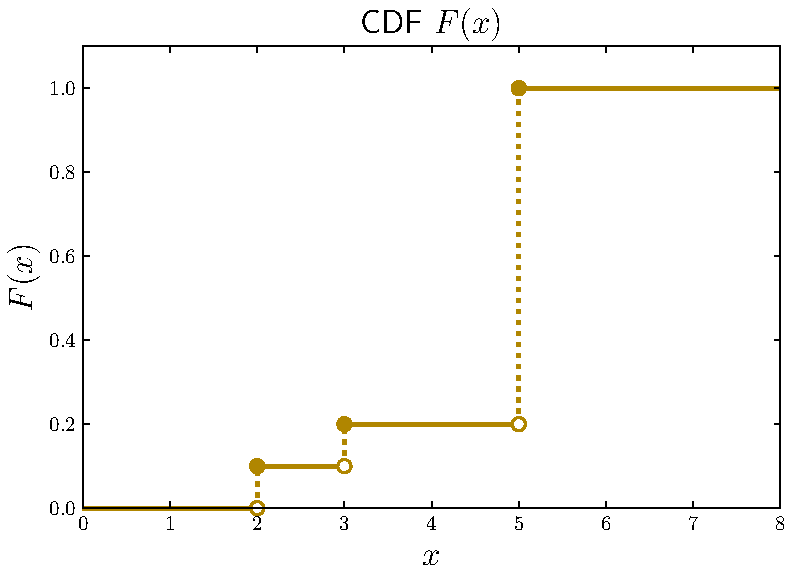
\includegraphics[width=1.0\textwidth]{chap2/chap2ex2.eps}
\end{center}

And the respective probabilities are
\begin{align*}
	\Prob(2 < X \le 4.8) & = \Prob(X \le 4.8) - \Prob(X \le 2) \\
	 & = 2/10 - 1/10 \\
	 & = \boxed{1/10} \\
	\Prob(2 \le X \le 4.8) & = \Prob(X \le 4.8) - \Prob(X < 2) \\
	 & = 2/10 - 0 \\
	 & = \boxed{1/5}
\end{align*}

% QUESTION 3
\qs{2.14.3}{Prove Lemma 2.15.}
\lemma{(Wasserman 2.15)}{Let \(F\) be the \textsf{CDF} for a random variable \(X\). Then:
\begin{enumerate}[label*=\arabic*.]
	\item \(\Prob(X = x) = F(x) - F(x^{-})\) where \(F(x^{-}) = \lim_{y \uparrow x} F(y)\); 
	\item \(\Prob(x < X \le y) = F(y) - F(x)\);
	\item \(\Prob(X > x) = 1 - F(x)\) ;
	\item If \(X\) is continuous then
		\begin{align*}
			F(b) - F(a) & = \Prob(a < X < b) = \Prob(a \le X < b) \\
			 & = \Prob(a < X \le b) = \Prob(a \le X \le b). \\
		\end{align*}
\end{enumerate}}
\begin{proof}[Proof]
	1. Let \(F(x^{-}) = \lim_{y \uparrow x } F(y) \). Then let \(y_{1}, y_{2}, \dots\) be a sequence such that \(y_{1} < y_{2} < \cdots\) and \(\lim_{i} y_{i} = x \). Then let \(A_{i} = (-\infty, y_{i}]\) and \(A = (-\infty, x]\), so \(A = \bigcup_{i=1}^{\infty} A_{i}\) and \(A_{1} \subset A_{2} \subset \cdots \). Thus by continuity of probability, \(\lim_{i} \Prob(A_{i}) = \Prob(\bigcup_{i} A_{i}) = \Prob(A) = F(x) \). But \(\lim_{i} \Prob(A_{i}) = F(x^{-})\) by definition, so we have \(F(x) = F(x^{-})\), implying \(\Prob(X = x) = F(x) - F(x^{-}) = 0\).
	\vspace{12pt}
	\par 2. We have \(\Prob(X \le y) = F(y)\) and \(\Prob(X \le x) = F(x)\). Using mutual exclusivity of the events \(\{\, X \colon X \le x\,\} \text{ and } \{\, X \colon x < X \le y \,\}, \) we can conclude that \(\Prob(X \le x) + \Prob(x < X \le y) = \Prob(X \le y)\) implies \(\Prob(x < X \le y) = F(y) - F(x)\).
\vspace{12pt}
	\par 3. By mutual exclusivity of the events \(\{\,X \colon X > x \,\} \text{ and } \Prob(X \le x)\), we must have \(\Prob(X \le x) + \Prob(X > x) = 1 \), which implies \(\Prob(X > x) = 1 - \Prob(X \le x) = 1 - F(x)\).
\vspace{12pt}
\par 4. Assume \(X\) is continuous. Then \(\Prob(X = a) = \Prob(X = b) = 0\). Since the events \(\{X = a\}, \{\, X \colon a < X < b \,\}, \{X = b \}\) are all disjoint, the desired equalities can be derived from summing the probabilities of the corresponding mutually exclusive events.
\end{proof}

\newpage
% QUESTION 4
\qs{2.14.4}{Let \(X\) have the probability density function
\[
	f_X(x) = \begin{cases}
		1/4  & 0 < x < 1 \\
		3/8  & 3 < x < 5 \\
		0    & \text{otherwise.}
	\end{cases}
\]
\begin{enumerate}[label=(\alph*)]
	\item Find the cumulative distribution function of \(X\).
	\item Let \(Y = 1/X\). Find the probability density function \(f_Y(y)\) for \(Y\). Hint: Consider three cases \(\frac{1}{5} \le y \le \frac{1}{3}, \frac{1}{3} \le y \le 1, \text{ and } y \ge 1.\)
\end{enumerate}
}
(a) To find the \textsf{CDF}, we find how the area under the \textsf{PDF} changes as \(x\) increases. The direct approach is to integrate each segment of the piecewise \textsf{PDF}, with some nuance -- as \(x\) moves between 1 and 3, since the \textsf{PDF} is zero here, there is no contribution to the \textsf{CDF}, and so \(F(x)\) stays at \(1/4\) on this segment. Additionally, once we reach the \((3,5)\) segment, we not only integrate \(3/8\) over the aforementioned interval, but add \(1/4\) to reflect the \textit{cumulative} probability. Proceeding in this manner, the \textsf{CDF} is
\[
	F_X(x) = \begin{cases}
		0 & x \le 0 \\
		x/4 & 0 < x < 1 \\
		1/4 & 1 \le x \le 3 \\
		1/4 + 3(x-3)/8 & 3 < x < 5 \\
		1 & 5 \le x	
	\end{cases} 
\]
Graphing the \textsf{PDF} and \textsf{CDF}:

\begin{center}
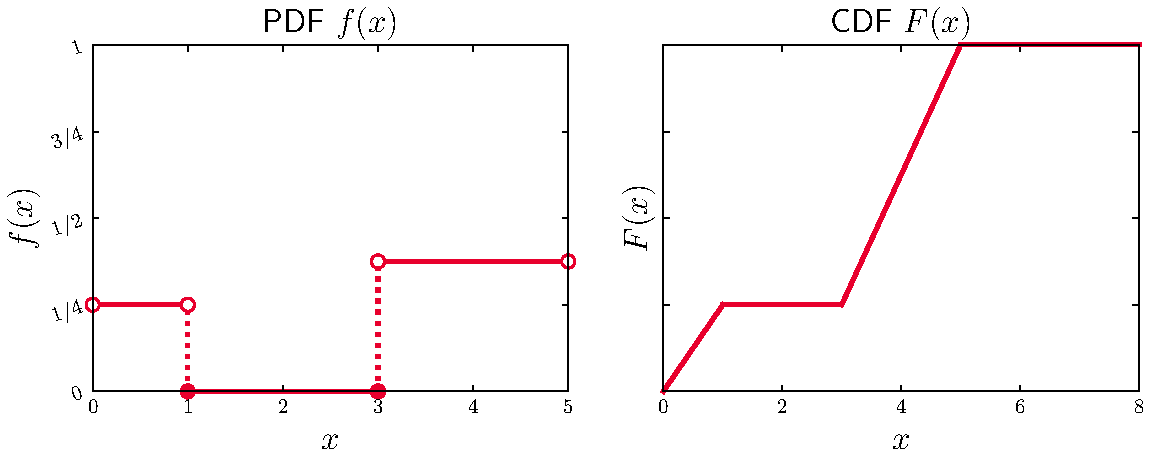
\includegraphics[width=1.0\textwidth]{chap2/chap2ex4a.eps}
\end{center}
\vspace{12pt}
	\par (b) To derive \(F_Y(y)\), we begin with
	\begin{align*}
		F_Y(y) & = \Prob(Y \le y) \\
		 & = \Prob(1/X \le y) \\
		 & = \Prob(1/y \le X) \\
		 & = 1 - \Prob(X < 1/y)
	\end{align*}

Since \(f_X(x)\) is given as a piecewise function, we must calculate the segments of the \textsf{CDF} \(F_Y(y)\), and consequently the \textsf{PDF} \(f_Y(y)\), separately.

Note also that
\[
	\frac{d}{dy} F_Y(y) = f_Y(y)
\]

\underline{Case 1:} \(1/5 < y < 1/3\) corresponding to \(3 < x < 5\)
\begin{align*}
	F_Y(y) & = 1 - \Prob(X < 1/y) \\
	 & = 1 - \left(\frac{1}{4} + \frac{3(1/y - 3)}{8} \right)   \\
	 & = \frac{15}{8} - \frac{3}{8y} \\
	\implies f_Y(y) & = \boxed{\frac{3}{8y^{2}}}
\end{align*}

\underline{Case 2:} \(1/3 \le y \le 1\) corresponding to \(1 \le x \le 3\)
\begin{align*}
	F_Y(y) & = 1 - \Prob(X < 1/y) \\
	 & = 1 - 1/4 \\
	 & = 3/4 \\
	\implies f_Y(y) & = \boxed{0}
\end{align*}

Intuitively, since \(f_X(x) = 0\) here, \(f_Y(y) = \boxed{0}\).

\underline{Case 3:} \(y > 1\) corresponding to \(0 < x < 1\)
\begin{align*}
	F_Y(y) & = 1 - \Prob(X < 1/y) \\
	 & = 1 - \frac{1}{4y} \\
	\implies f_Y(y) & = \boxed{\frac{1}{4y^{2}}}
\end{align*}
Thus the \textsf{CDF} and \textsf{PDF} of \(Y\) is given by
\[\begin{aligned}
	F_Y(y) & = \begin{cases}
		0 & y \le 1/5 \\
		15/8 - 3/8y & 1/5 < y < 1/3 \\
		3/4 & 1/3 \le y \le 1 \\
		1 - 1/4y & y > 1 
	\end{cases} \\
	f_Y(y) & = \begin{cases}
		3/8y^{2} & 1/5 < y < 1/3 \\
		1/4y^{2} & y > 1 \\
		0 & \text{otherwise}	
	\end{cases}
 \end{aligned}
\]
Graphing the \textsf{PDF} and \textsf{CDF}:
\begin{center}
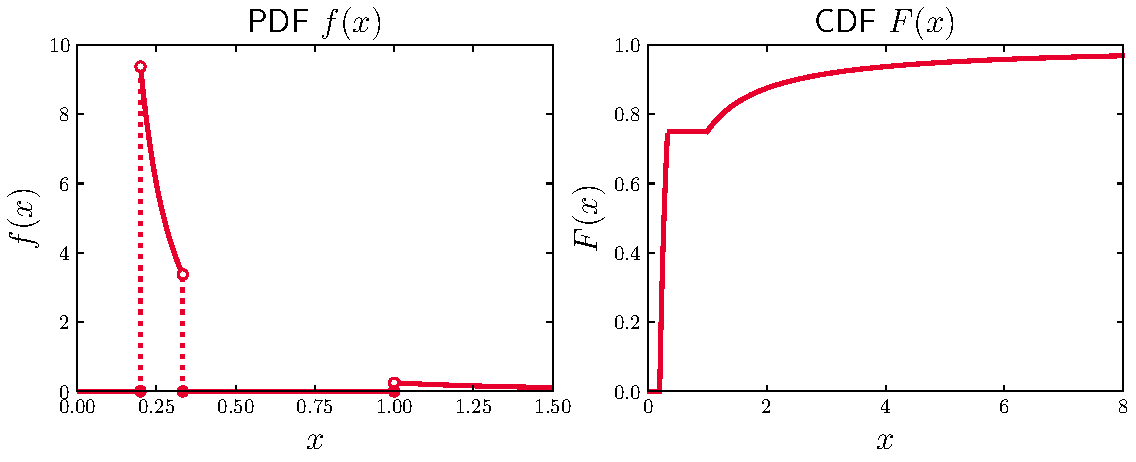
\includegraphics[width=1.0\textwidth]{chap2/chap2ex4b.eps}
\end{center}

% QUESTION 5
\qs{2.14.5}{Let \(X\) and \(Y\) be discrete random variables. Show that \(X\) and \(Y\) are independent if and only if \(f_{X,Y}(x,y) = f_{X}(x)f_{Y}(y)\) for all \(x\) and \(y\).}
\begin{proof}[Proof] 
\((\implies)\) Let \(X \sqcup Y\). Then for all \(x, y\), \(\Prob(X = x, Y=y) = \Prob(X = x)\Prob(Y = y)\). Since \(f_X(x) = \Prob(X = x), f_Y(y) = \Prob(Y = y)\), and \(f_{X,Y}(x,y) = \Prob(X = x, Y = y)\), we have
\[
	f_{X,Y}(x,y) = f_{X}(x)f_{Y}(y)
\]
\par \( (\impliedby) \) Let \(f_{X,Y}(x,y) = f_{X}(x)f_{Y}(y)\) for all \(x, y\). Since \(f_{X,Y}(x,y) = \Prob(X=x, Y=y)\), \(f_{X}(x) = \Prob(X=x)\) and \(f_{Y}(y) = \Prob(Y=y)\), we must have
\[
	\Prob(X=x, Y=y) = \Prob(X=x)\Prob(Y=y)
\]
for all \(x,y\). Thus \(X \sqcup Y\).
\end{proof}

% QUESTION 6
\qs{2.14.6}{Let \(X\) have distribution \(F\) and density function \(f\) and let \(A\) be a subset of the real line. Let \(I_{A}(x)\) be the indicator function for \(A\):
\[
	I_{A}(x) = \begin{cases}
		1 & x \in  A \\
		0 & x \not\in A. \\
	\end{cases}
\]
Let \(Y = I_{A}(X)\). Find an expression for the cumulative distribution of \(Y\). (Hint: first find the probability mass function for \(Y\).)}
Let \(Y = I_{A}(x)\). Then
\[
	f_{Y}(y) = \begin{cases}
		\Prob(Y = 1) = \int_{A} f \ dx & x \in A \\
		\Prob(Y = 0) = 1 - \int_{A} f \ dx & x \not\in A \\
		0 & \text{otherwise}
	\end{cases}
\]
which implies
\[
	F_{Y}(y) = \begin{cases}
		0 & y < 0 \\
		1 - \int_{A} f \ dx  & 0 \le y < 1 \\
		1 & y \ge 1 \\
	\end{cases}
\]
% QUESTION 7
\qs{2.14.7}{Let \(X\) and \(Y\) be independent and suppose that each has a \(\Uniform(0,1)\) distribution. Let \(Z = \min\{X,Y\}\). Find the density \(f_{Z}(z)\) for \(Z\). Hint: It might be easier to first find \(\Prob(Z > z)\).}

One can follow the hint and observe that \(\Prob(Z > z)\) if and only if 
\[
	\Prob(X > z)\Prob(Y > z) = (1 - \Prob(X < z))(1 - \Prob(Y < z)) = (1 - F_{X}(z))(1 - F_{Y}(z))
\]
and applying the fact that \(F_{X}(x), F_{Y}(y)\) both follow a standard uniform distribution. We will also attempt to derive the density \(f_{Z}(z)\) by modeling the mutual exclusivity of either \(X\) or \(Y\) being the minimum.

We define \(Z\) as
\[
	Z = \min\{X,Y\} = \begin{cases}
		X & x < y \\
		Y & y < x \\
	\end{cases} 
\]
Since \(X,Y\) have standard uniform distribution, it must also be the case that \(0 < z < 1\) has non-zero probability, and zero probability otherwise.

Our task is to derive \(\Prob(0 < Z < z)\). Either \(X \le Y\) or \(Y \le X\), and in those cases, we must also have \(X \le z\) and \(Y \le z\), respectively. Thus we derive \(F_{Z}(z)\) on this interval:
\begin{align*}
	\Prob(0 < Z \le z) & = \Prob(X \le z)\Prob(X \le Y) + \Prob(Y \le z)\Prob(Y \le X) \\
	 & = \int^{z}_{0} \int^{1}_{x}  \ dy  \ dx + \int^{z}_{0} \int^{1}_{y}  \ dx  \ dy  \\
	 & = \boxed{2z - z^{2}}
\end{align*}
Similarly, we look at \(\Prob(z < Z < 1)\), which corresponds to \(1 - F_{Z}(z)\). As in the previous case, either \(X \le Y\) or \(Y \le X\), but this time these cases correspond to \(X > z\) and \(Y > z\). We derive
\begin{align*}
	\Prob(z < Z < 1) & = \Prob(X > z)\Prob(X \le Y) + \Prob(Y > z)\Prob(Y \le X) \\
	 & = \int^{1}_{z} \int^{1}_{x}  \ dy  \ dx + \int^{1}_{z} \int^{1}_{y}  \ dx  \ dy  \\
	 & = \boxed{1 - 2z + z^{2}}
\end{align*}
Either way, we can conclude
\begin{align*}
	F_{Z}(z) & = \begin{cases}
		0 & z \le 0 \\
		2z - z^{2} & 0 < z < 1 \\
	        1 & z \ge 1
	\end{cases} \\
	f_{Z}(z) & = \begin{cases}
		2(1-z) & 0 < z < 1  \\
		0 & \text{otherwise} \\
	\end{cases} \\
\end{align*}
And as anticipated, our theoretical work aligns with the empirical:
\begin{center}
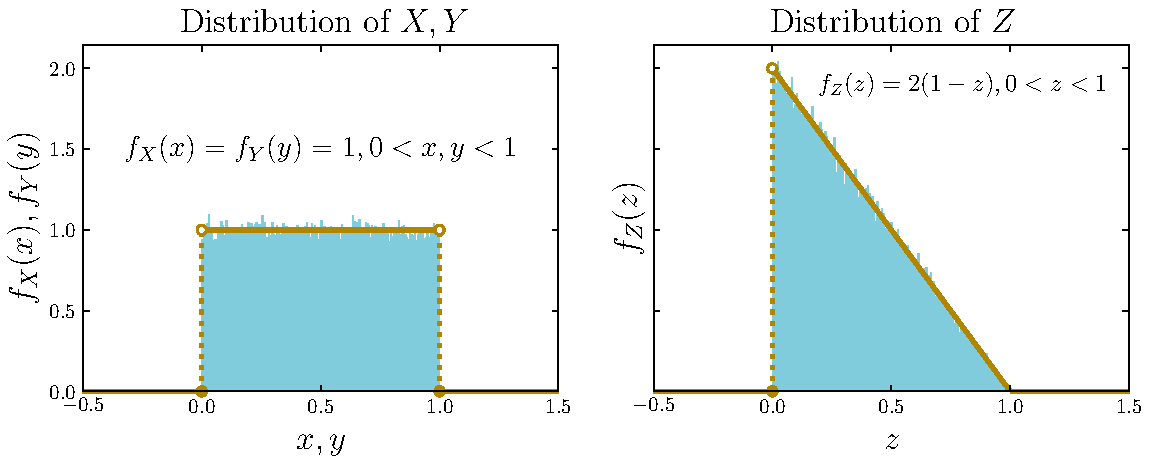
\includegraphics[width=1.0\textwidth]{chap2/chap2ex7.eps}
\end{center}

% QUESTION 8
\qs{2.14.8}{Let \(X\) have \textsf{CDF} \(F\). Find the \textsf{CDF} of \(X^{+} = \max\{0,X\}\).}
Observe that \(\Prob(X^{+} = 0) = \Prob(X \le 0) = F(0)\). For \(X > 0\), we have \(\Prob(X^{+} = X) = \Prob(0 < X \le x) = F(x) - F(0)\). Then the \textsf{CDF} of \(X^{+}\) is
\[
	F_{X^{+}}(X^{+}) = \begin{cases}
		F_{X}(0) & X \le 0, X^{+} = 0 \\
		F_{X}(x) & X > 0, X^{+} = X > 0 \\
	\end{cases}
\]

% QUESTION 9
\qs{2.14.9}{Let \(X \sim \Exp(\beta)\). Find \(F(x)\) and \(F^{-1}(q)\).}
\[
	F(x) = \int^{x}_{0} \frac{1}{\beta}\exp(-x/\beta) \ dx = 1 - \exp(-x/\beta),\quad x > 0 \\
\]
Let \(q = F(x)\). Then \(q = 1 - \exp(-x/\beta )\) implies
\begin{align*}
	\implies & \exp(-x/\beta ) = 1-q \\
	\implies & \boxed{x = -\beta \ln(1-q)}, \quad 0 \le q < 1
\end{align*}

% QUESTION 10
\qs{2.14.10}{Let \(X\) and \(Y\) be independent. Show that \(g(X)\) is independent of \(h(Y)\) where \(g\) and \(h\) are functions.}
\begin{proof}[Proof] 
Let \(X \sqcup Y\). Consider the joint probability \(\Prob(X,Y)\). By premise, \(\Prob(X,Y) = \Prob(X)\Prob(Y)\) for all \(x,y\). Now consider \(g(X), h(Y)\). Let 
\begin{align*}
	A & = \{\, X \colon g(X) \in A' \,\} \\
	B & = \{\, Y \colon h(Y) \in B'\,\}
\end{align*}
where \(A', B'\) are the sets containing the respective transformations of \(X \in A, Y \in B\). The intuition to have here is that the "link" between \(X \in A\) and \(g(X) \in A'\) preserves the independence of the former in the latter under transformation.

Then we have
\begin{align*}
	\Prob(g(X) \in A') & = \Prob(X \in A) \\
	\Prob(h(Y) \in B') & = \Prob(Y \in B) \\
	\implies \Prob(g(X) \in A', h(Y) \in B') & = \Prob(X \in A, Y \in B)
\end{align*}
Applying independence on the last equality,
\[
	\Prob(g(X \in A'), h(y \in B')) = \Prob(g(X \in A'))\Prob(h(Y \in B'))	
\]
ascertaining that \(g(X) \sqcup h(X)\).
\end{proof}

% QUESTION 11
\qs{2.14.11}{Suppose we toss a coin once and let \(p\) be the probability of heads. Let \(X\) denote the number of heads and let \(Y\) denote the number of tails.
\begin{enumerate}[label=(\alph*)]
	\item Prove that \(X\) and \(Y\) are dependent.
	\item Let \(N \sim \Poisson(\lambda)\) and suppose we toss a coin \(N\) times. Let \(X\) and \(Y\) be the number of heads and tails. Show that \(X\) and \(Y\) are independent.
\end{enumerate}}
\begin{proof}[Proof] 
(a) We have \(\Prob(X=1) = p\) and \(\Prob(Y=1) = 1-p\), where \(X,Y\) are the number of heads and tails. Note that \(\Prob(X=1,Y=1) = 0\), as we can only have one head or one tail after a single toss. But clearly \(\Prob(X=1)\Prob(Y=1) = p(1-p) = 0\) for non-zero \(p\), so \(X, Y\) are dependent.
\vspace{12pt}
\par (b) The intuition is to decompose the joint probability \(f_{X,Y}(x,y)\) into \(g(x)h(y)\), where \(g(x), h(y)\) are \textit{any} functions (not necessarily densities). We can equivalently find the joint probability that we toss \(X = x\) heads \textit{and} toss the coin \(N\) times:
\begin{align*}
	\Prob(X = x, Y = y) & = \Prob(X = x, N = x+y) \\
			    & = \binom{N}{x} p^{x}(1-p)^{N-x}e^{-\lambda} \frac{\lambda^{N}}{N!} \\
			    & = \binom{x+y}{x} p^{x}(1-p)^{y} e^{-\lambda} \frac{\lambda^{x+y}}{(x+y)!} \\
			    & = \frac{(x+y)!}{x!y!} p^{x}(1-p)^{y}e^{-\lambda} \frac{\lambda^{x+y}}{(x+y)!} \\
			    & = \underbrace{\left(e^{-\lambda} \frac{\lambda^{x}}{x!}p^{x}  \right)}_{g(x)} \underbrace{\left( \frac{\lambda^{y}}{y!} (1-p)^{y} \right) }_{h(y)} 
\end{align*}
\end{proof}

\newpage
% QUESTION 12
\qs{2.14.12}{Prove Theorem 2.33.}
\thm{(Wasserman 2.33)}{Suppose that the range of \(X\) and \(Y\) is a (possibly infinite) rectangle. If \(f(x,y) = g(x)h(y)\) for some functions \(g\) and \(h\) (not necessarily probability density functions) then \(X\) and \(Y\) are independent.}
\begin{proof}[Proof] 
Let \(X, Y\) have density \(f(x,y)\), and define
\[
	A = \{\,(x,y) \colon x > 0, y > 0 \,\}
\]
Then
\begin{align*}
	1 & = \int \int_{A} f(x,y)  \ dx  \ dy  \\
	  & = \underbrace{\int^{\infty}_{0} g(x) \ dx}_{c} \underbrace{\int^{\infty}_{0} h(y) \ dy }_{1/c}
\end{align*}
where \(0 < c < 1\). Let \(f_{X}(x) = \frac{1}{c} g(x), x > 0\) and \(f_{Y}(y) = ch(y), y > 0\). Then
\[
	f(x,y) = g(x)h(x) = \left( \frac{1}{c} g(x) \right) \left( c h(y) \right) = f_{X}(x) f_{Y}(y)
\]
for all \(x, y\). Thus \(X \sqcup Y\).
\end{proof}

% QUESTION 13
\qs{2.14.13}{Let \(X \sim N(0,1\) and let \(Y = e^{X}\).
\begin{enumerate}[label=(\alph*)]
	\item Find the \textsf{PDF} for \(Y\). Plot it.
	\item \textsf{(Computer Experiment.)} Generate a vector \(x = (x_{1},\dots, x_{10,000})\) consisting of \(10,000\) random standard Normals. Let \(y = (y_{1},\dots, y_{10,000})\) where \(y_{i} = e^{x_{i}}\). Draw a histogram of \(y\) and compare it to the \textsf{PDF} you found in part (a).
\end{enumerate}}
\begin{align*}
	F_{Y}(y) & = \Prob(Y \le y) \\
	 & = \Prob(e^{X} \le y) \\
	 & = \Prob(X \le \ln y) \\
	 & = \frac{1}{\sqrt{2\pi}} \int^{\ln y}_{-\infty} \exp \left( -\frac{x^{2}}{2} \right)  \ dx \\
	 & = \frac{1}{\sqrt{2\pi}} \int^{0}_{-\infty} \exp \left( -\frac{x^{2}}{2} \right)  \ dx + \frac{1}{2\pi} \int^{\ln y}_{0} \exp \left( -\frac{x^{2}}{2} \right)  \ dx  
\end{align*}
Applying the Leibniz rule, we find
\[
	F_{Y}'(y) = f_{Y}(y) = \frac{1}{y\sqrt{2 \pi}}  \exp \left( -\frac{1}{2} (\ln y)^{2} \right), \quad y > 0
\]
\vspace{12pt}
\par (b) Our theoretical and empirical results agree:
\begin{center}
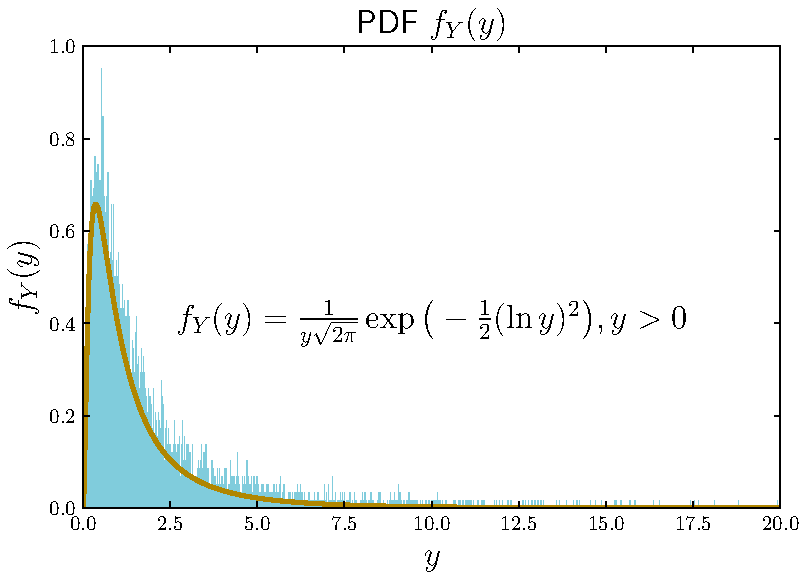
\includegraphics[width=1.0\textwidth]{chap2/chap2ex13.eps}
\end{center}

% QUESTION 14
\qs{2.14.14}{Let \((X,Y)\) be uniformly distributed on the unit disk \(\{\,(x,y) \colon x^{2} + y^{2} \le 1 \,\}\). Let \(R = \sqrt{X^{2}+Y^{2}}\). Find the \textsf{CDF} and \textsf{PDF} of \(R\).}

For a joint density involving uniformly distributed variables, \(f(x,y) = 1/\text{area}(A)\), where \(A\) is the region over which the densities of the constituent variables are defined and non-zero. Since we choose uniformly distributed \((x,y)\) over the unit circle, its area is \(A = \pi \).

Integrating in polar coordinates, we derive for \(0 < r < 1\):
\[
	F_{R}(r) = \int^{2 \pi }_{0} \int^{r}_{0} \frac{1}{\pi }s \ ds   \ d \theta = \int^{2 \pi }_{0} \frac{1}{\pi }\frac{r^{2}}{2} \ d\theta = r^{2} 
\]
giving us the \textsf{CDF} and \textsf{PDF}:
\begin{align*}
	F_{R}(r) & = \begin{cases}
		0 & r \le 0 \\
		r^{2} & 0 < r <  \\
	        1 & r \ge 1
	\end{cases} \\
	F'_{R}(r) = f_{R}(r) & = 2r, \quad 0 < r < 1 \\
\end{align*}

Empirically generating the \((x,y)\)'s agrees with the theoretically derived density:
\begin{center}
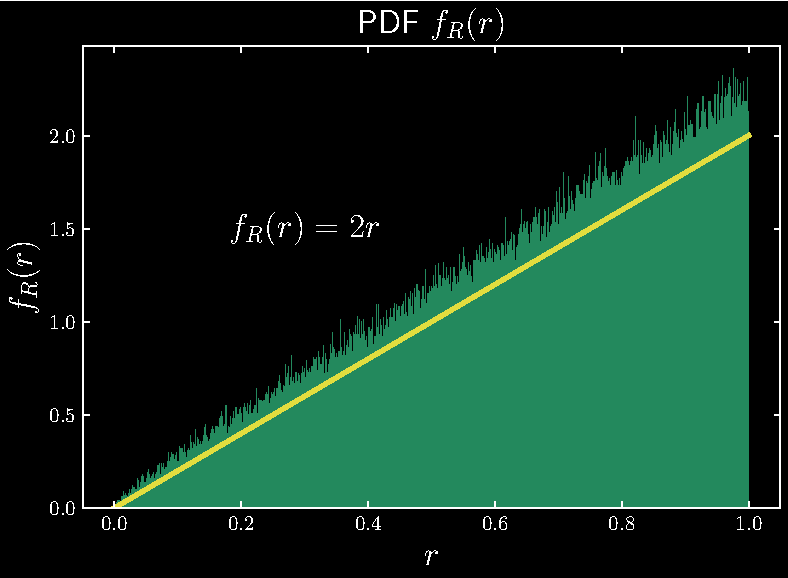
\includegraphics[width=1.0\textwidth]{chap2/chap2ex14.eps}
\end{center}

% QUESTION 15
\qs{2.14.15}{\textsf{(A universal random number generator.)} Let \(X\) have a continuous, strictly increasing \textsf{CDF} \(F\). Let \(Y = F(X)\). Find the density of \(Y\). This is called the probability integral transform. Now let \(U \sim \Uniform(0,1)\) and let \(X = F^{-1}(U)\). Show that \(X \sim F\). Now write a program that takes \(\Uniform(0,1)\) random variables and generates random variables from an \(\Exp(\beta )\) distribution.}
\begin{proof}[Proof] 
By assumption, \(F_{X}(x)\) is strictly increasing and continuous. This means \(F_{X}(x)\) is a bijection, and has an inverse \(F_{X}^{-1}(x)\). We use this fact to derive
\begin{align*}
	F_{Y}(y) & = \Prob(Y \le y) \\
	 & = \Prob(F_{X}(x) \le y) \\
	 & = F_{X}(F_{X}^{-1}(y)) \\
	 & = y \\
	\implies F_{Y}^{-1}(y) = f_{Y}(y) & = 1
\end{align*}

A shocking result! All probability integral transforms of \textit{any} continuous distribution give us the density to the standard uniform distribution. 

For the next result, let \(U \sim \Uniform(0,1)\) and \(X = F^{-1}(U)\). The intuition to have here is that \(F^{-1}\) is a quantile function! Again appealing to the bijectivity of \(F\), we have \(F(X) = U\). Since \(F: X \rightarrow [0,1]\) and invoking the preservation of monotonocity under an inverse operation \((x_{1} < x_{2} \iff F(x_{1}) < F(x_{2}))\), we have 
\[
	\Prob(X \le x) = \Prob(F^{-1}(U) \le x) = \Prob(U \le F(x)) = F(x)
\]
Thus we must have \(X \sim F\).
\end{proof}

The quantile function for the \(\Exp(\beta )\) distribution is \(F^{-1}(q) = -\beta \ln(1-q)\). Generating the exponential distribution via the probability integral transform:

\begin{center}
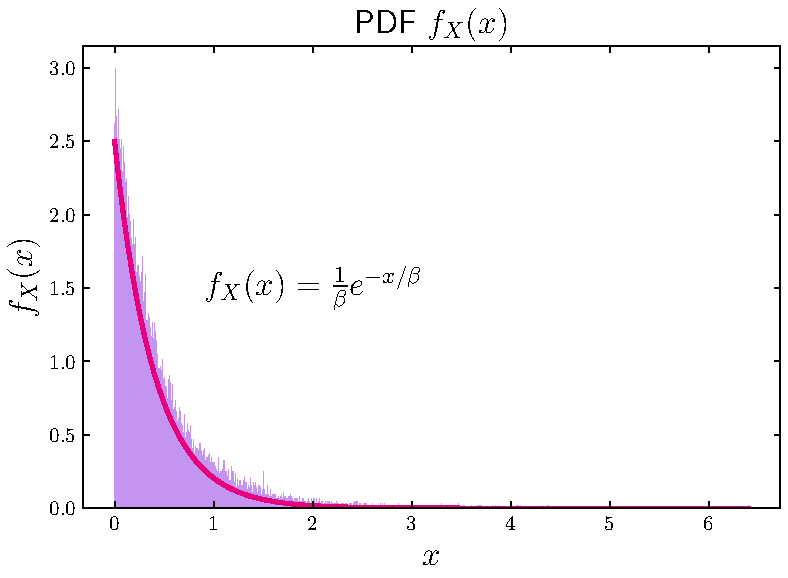
\includegraphics[width=1.0\textwidth]{chap2/chap2ex15.eps}
\end{center}

% QUESTION 16
\qs{2.14.16}{Let \(X \sim \Poisson(\lambda )\) and \(Y \sim \Poisson(\mu)\) and assume that \(X\) and \(Y\) are independent. Show that the distribution of \(X\) given that \(X + Y = n\) is \(\binomial(n,\pi )\) where \(\pi = \lambda / (\lambda + \mu)\).

Hint 1: You may use the following fact: If \(X \sim \Poisson(\lambda )\) and \(Y \sim \Poisson(\mu)\), and \(X\) and \(Y\) are independent, then \(X + Y \sim \Poisson(\mu + \lambda )\).

Hint 2: Note that \(\{X = x, X + Y = n \} = \{X = x, Y = n-x \}\).}
\begin{proof}[Proof] 
By definition of the Poisson distribution:
\begin{align*}
	f(X+Y = n) & = e^{-(\lambda + \mu)} \frac{(\lambda + \mu)^n}{n!} \\
	f(X = x, Y = n-x) & = e^{-\lambda } \frac{\lambda^{x}}{x!} e^{-\mu} \frac{\mu^{n-x}}{(n-x)!}
\end{align*}
Proceeding to set up the conditional probability:
\begin{align*}
	f(X  \mid  X + Y = n) & = \frac{e^{-\lambda } \frac{\lambda^{x}}{x!} e^{-\mu} \frac{\mu^{n-x}}{(n-x)!}}{e^{-(\lambda + \mu)} \frac{(\lambda + \mu)^n}{n!}} \\
			 & = \frac{\lambda^{x} \mu^{n-x}}{(\lambda + \mu)^{n}} \frac{n!}{(n-x)!x!} \\
			 & = \binom{n}{x} \left( \frac{\lambda }{\lambda + \mu} \right)^{x} \left( \frac{\mu}{\lambda + \mu} \right)^{n-x} \\
			 & = \binom{n}{x} \left( \frac{\lambda }{\lambda + \mu} \right)^{x} \left( 1 - \frac{\lambda }{\lambda + \mu} \right)^{n-x}  
\end{align*}
ascertaining that \(X  \mid  X + Y = n \sim \binomial(n,\pi )\) for \(\pi = \lambda / (\lambda + \mu)\).
\end{proof}

% QUESTION 17
\qs{2.14.17}{Let
\[
	f_{X,Y}(x,y) = \begin{cases}
		c(x+y^{2}) & 0 \le x < 1 \text{ and } 0 \le y \le 1 \\
		0 & \text{otherwise.} \\
	\end{cases}
\]
Find \(\Prob(X < \frac{1}{2}  \mid  Y = \frac{1}{2})\).}

First we find the marginal density function of \(y\):
\[
	f_{Y}(y) = \int^{1}_{0} c(x+y^{2}) \ dx = c(1/2 + y^{2})
\]
Then the conditional density function is
\[
	f_{X \mid Y}(x \mid y) = \frac{x + y^{2}}{1/2 + y^{2}}
\]
Now we calculate the desired probability:
\begin{align*}
	\Prob(X < 1/2  \mid  Y = 1/2) & = \int^{1/2}_{0}  f_{X \mid Y}(x  \mid  1/2) \ dx  \\
	 & = \int^{1/2}_{0} \frac{x + 1/4}{1/2 + 1/4} \ dx  \\
	 & = \frac{1/8 + 1/8}{1/2 + 1/4} \\
	 & = \boxed{1/3}
\end{align*}

\newpage
% QUESTION 18
\qs{2.14.18}{Let \(X \sim N(3,16)\). Solve the following using the Normal table and using a computer package.
\begin{enumerate}[label=(\alph*)]
	\item Find \(\Prob(X < 7)\).
	\item Find \(\Prob(X > -2)\).
	\item Find \(x\) such that \(\Prob(X > x) = .05\).
	\item Find \(\Prob(0 \le X < 4)\).
	\item Find \(x\) such that \(\Prob( \mid X \mid  >  \mid x \mid ) = .05\).  
\end{enumerate}}
It is best to use scipy.stats here:

Using the above calculations:

\begin{enumerate}[label=(\alph*)]
	\item \(\Prob(X < 7) = 0.841\)
	\item \(\Prob(X > -2) = 0/894\)
	\item \(x = 9.579\)
	\item \(\Prob(0 \le X < 4) = 0.372\)
	\item \(x = 9.611\)
\end{enumerate}

For (e), the intuition behind the absolute values is to evaluate the probabilities at the tails of the distribution. Given \( \mid x \mid  > 0\), we can equivalently write
\begin{align*}
	\Prob( \mid X \mid  >  \mid x \mid ) & = \Prob(X >  \mid x \mid ) + \Prob(X < - \mid x \mid ) \\
	 & = 1 - \Prob(X <  \mid x \mid ) + \Prob(X < - \mid x \mid ) = 0.05 \\
	\implies 0.95 & = \Prob(X <  \mid x \mid ) - \Prob(X < - \mid x \mid )
\end{align*}

Numerically iterating enables us to identify the value of \( \mid x \mid  = x\) without needing to convert to a standard normal distribution.

% QUESTION 19
\qs{2.14.19}{Prove formula (2.12).}
\prp{(Wasserman Formula 2.12)}{For a strictly monotone increasing or strictly monotone decreasing function \(r(X)\) with an inverse \(s = r^{-1}\), we have
\[
	f_{Y}(y) = f_{X}(s(y)) \bigg| \frac{d s(y) }{d y}  \bigg| .
\]}
\begin{proof}[Proof] 
\underline{Case 1: Increasing \(r(X).\)} Derive
\begin{align*}
	F_{Y}(y) = \Prob(Y \le y) & = \Prob(r(X) \le y) \\
	 & = \Prob(X \le r^{-1}(y)) \\
	 & = \Prob(X \le s(y)) \\
	 & = \int^{s(y)}_{-\infty} f_{X}(x) \ dx 
\end{align*}
Implying \(F'_{Y}(y) = f_{Y}(y) = f_{X}(s(y)) \frac{d s(y)}{d y} \). Note that since \(r(X)\) is strictly monotone increasing by premise, \(ds(y)/dy > 0\).
\vspace{12pt}
\par \underline{Case 2: Decreasing \(r(X)\).} Derive
\begin{align*}
	F_{Y}(y) = \Prob(Y \le y) & = \Prob(r(X) \le y)  \\
	 & = \Prob(X \ge r^{-1}(y)) \\
	 & = \Prob(X \ge s(y)) \\
	 & = 1 - \Prob(X \le s(y)) \\
	 & = 1 - \int^{s(y)}_{-\infty} f_{X}(x) \ dx \\
	F'_{Y}(y) = f_{Y}(y) & = - f_{X}(s(y)) \frac{d s(y)}{d y} 
\end{align*}
where the second equality follows because \(r(X)\) is strictly monotonically \textit{decreasing}. That same fact also allows us to say that \(ds(y) / dy < 0\). To encapsulate both the increasing and decreasing cases, we have
\[
	f_{Y}(y) = f_{X}(s(y)) \bigg| \frac{d s(y)}{d y}  \bigg| 
\]
\end{proof}

% QUESTION 20
\qs{2.14.20}{Let \(X,Y \sim \Uniform(0,1)\) be independent. Find the \textsf{PDF} for \(X-Y\) and \(X/Y\).}

The joint probability density function is given by
\[
	f_{X,Y}(x,y) = \begin{cases}
		1 & 0 < x, y < 1 \\
		0 & \text{otherwise} \\
	\end{cases}
\]
\underline{\(X - Y\)}

\par Illustrations are particularly useful here to understand where the piecewise segments of \(f_{Z}(z)\) are defined.

Given \(Z = X-Y\), it must be the case that either \(0 < z < 1\) or \(-1 < z < 0\). To find \(A_{z}\), the support for the probability density function, we find all \(x, y\) satisfying
\[
	A_{z} = \{\,(x,y) \colon x - y \le z \,\}
\]
Now, there is a nice geometric intuition in that the piecewise \textsf{CDF} is given by the area of the support on each interval \(0 < z < 1, -1 < z < 0\). Graphically, this support in the first and second cases is:

\begin{center}
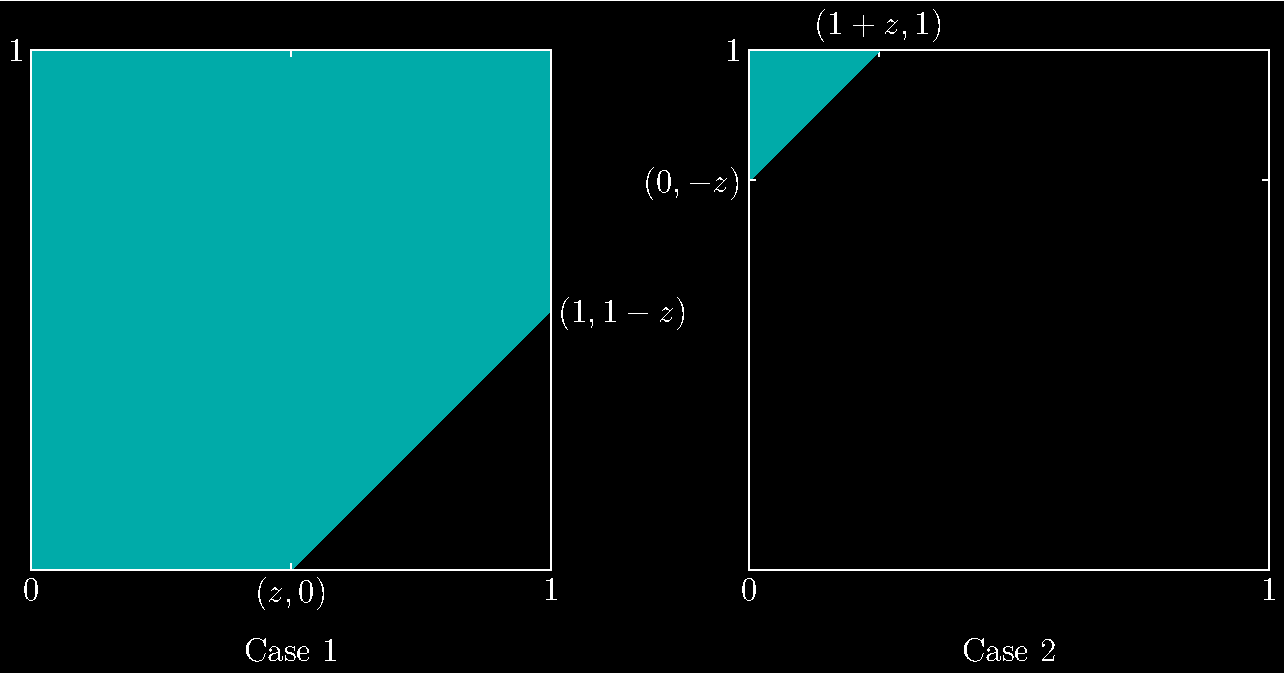
\includegraphics[width=1.0\textwidth]{chap2/chap2ex20i.eps}
\end{center}

Calculating the area of the shaded parts, we can derive the \textsf{CDF} as
\[
	F_{Z}(z) = \begin{cases}
		0 & z < -1 \\
		\frac{1}{2}(1+z)^{2} & -1 < z < 0 \\
		1 - \frac{1}{2}(1-z)^{2} & 0 < z < 1 \\
		1 & z > 1
	\end{cases}
\]
and consequently, the \textsf{PDF} is
\[
	f_{Z}(z) = \begin{cases}
		1 + z & -1 < z < 0 \\
		1 - z & 0 < z < 1 \\
		0 & \text{otherwise}
	\end{cases}
\]

which agrees with our empirical simulation:
\begin{center}
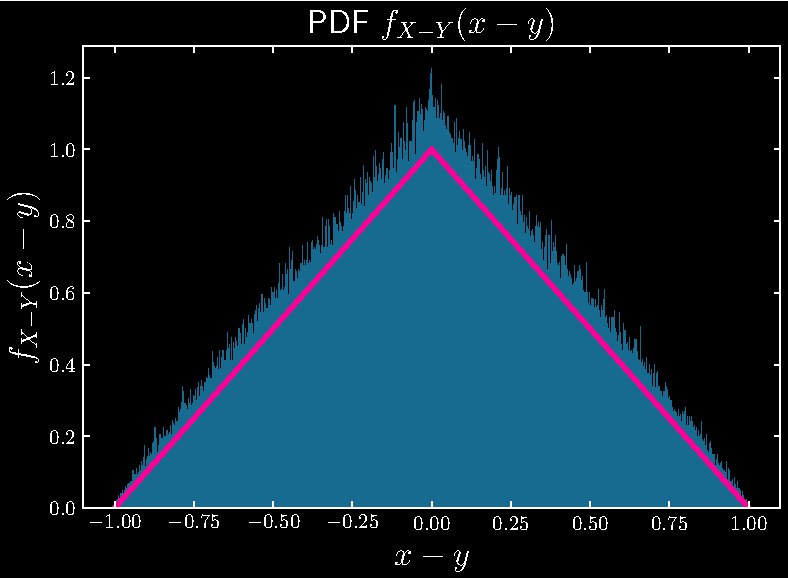
\includegraphics[width=1.0\textwidth]{chap2/chap2ex20iii.eps}
\end{center}

\underline{\(X/Y\)}
\par Once again finding the supports for \(Z = X/Y\), observe that the intervals we examine are \(0 < z < 1\) and \(z > 1\). The areas are graphed as

\begin{center}
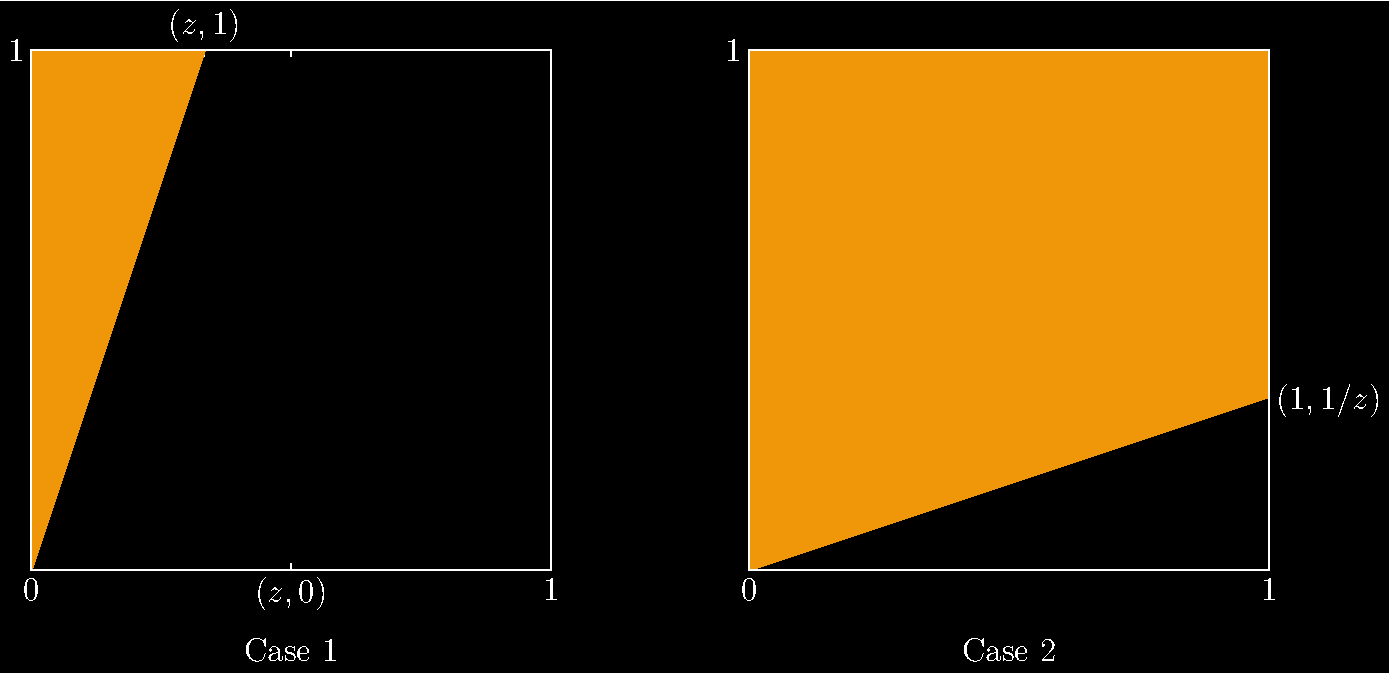
\includegraphics[width=1.0\textwidth]{chap2/chap2ex20ii.eps}
\end{center}

with \textsf{CDF}
\[
	F_{Z}(z) = \begin{cases}
		0 & z < 0 \\
		\frac{z}{2} & 0 < z < 1 \\
		1 - \frac{1}{2z} & z > 1
	\end{cases}
\]
and following that, the \textsf{PDF}
\[
	f_{Z}(z) = \begin{cases}
		\frac{1}{2} & 0 < z < 1 \\
		\frac{1}{2z^{2}} & z > 1 \\
		0 & \text{otherwise}
	\end{cases}
\]
Once again, the theoretical and the empirical align:
\begin{center}
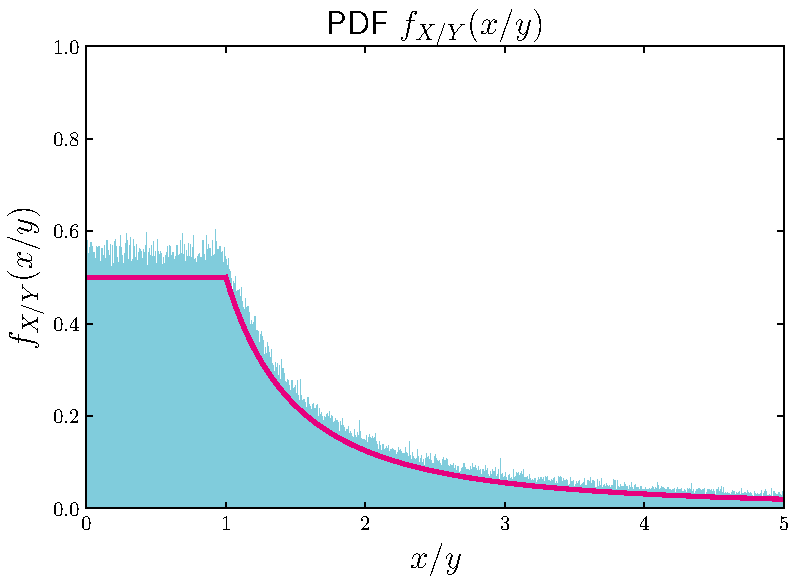
\includegraphics[width=1.0\textwidth]{chap2/chap2ex20iv.eps}
\end{center}

% QUESTION 21
\qs{2.14.21}{Let \(X_{1},\dots,X_{n} \sim \Exp(\beta )\) be \textsf{IID}. Let \(Y = \max\{X_{1},\dots,X_{n}\}\). Find the \textsf{PDF} of \(Y\). Hint: \(Y \le y\) if and only if \(X_{i} \le y\) for \(i = 1,\dots,n\).}

Taking advantage of the hint and the \textsf{IID} random variables, observe that \(\Prob(Y \le y) = \prod_{i=1}^{n} \Prob(X_{i} \le y) \). The derivation is straightforward:
\begin{align*}
	F_{Y}(y) = \Prob(Y \le y) & = \prod_{i=1}^{n} \int^{y}_{0} \frac{1}{\beta }e^{-x_{i}/\beta } \ dx_{i}   \\
	 & = \prod_{i=1}^{n} (1 - e^{-y/\beta })  \\
	 & = (1 - e^{-y/\beta })^{n} \\
	\implies F'_{Y}(y) = f_{Y}(y) = \frac{d }{d y} (1 - e^{-y/\beta })^{n} & = \boxed{\frac{n}{\beta } e^{-y/\beta }(1 - e^{-y/\beta })^{n-1}}
\end{align*}

\end{document}
